\chapter{VAR-Tool}
\label{ch:main-matter}
  \begin{figure}[H]
    \centering
    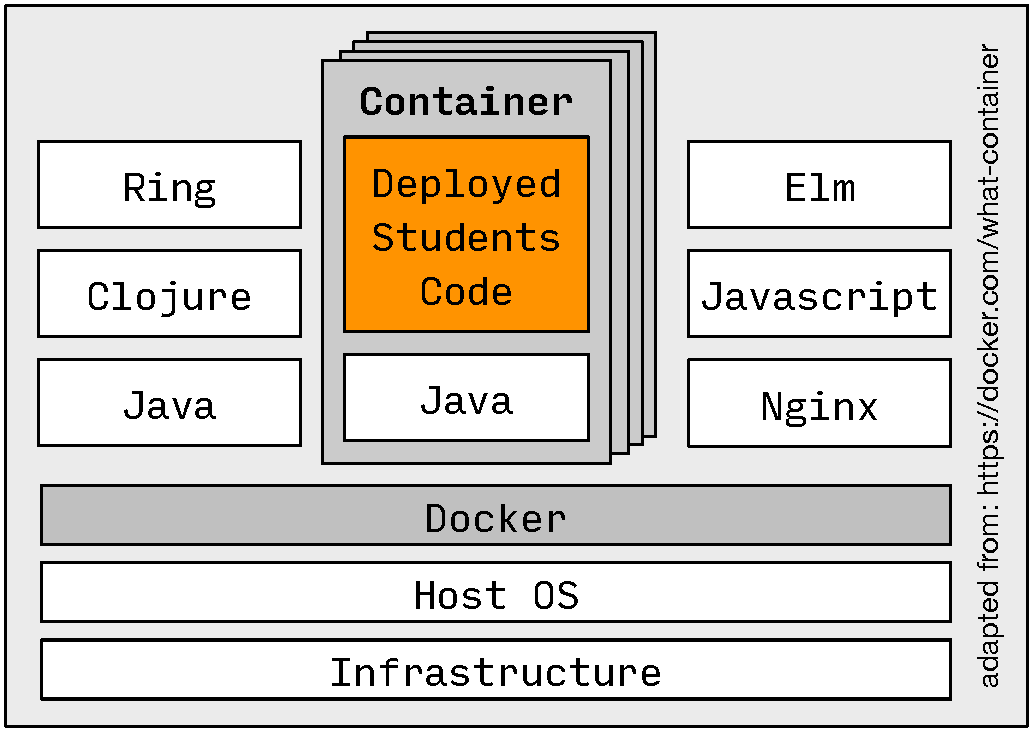
\includegraphics[scale=0.4]{container_intro_centered.pdf}
    \par
    \caption{Container-Übersicht}
    \label{fig:container-intro}
  \end{figure}
  Diese Kapitel beschreibt die Vorgehensweise und Umsetzung des VAR-Tools.
  Es wird zunächst ein Mockup des Clients vorgestellt und dann auf die weitere Architektur des Systems eigegangen.
  Abbildung~\ref{fig:container-intro} zeigt eine Übersicht der geplanten Applikation.
  Wir haben auf der linken Seite einen Server-Container, welcher auf Java bzw. Clojure aufgebaut ist.
  Daneben befinden sich mehrere User-Container in denen anschließend Programmpakete eines Studierenden ausgeliefert werden sollen.
  Auf der rechten Seite ist ein Client-Container sichtbar, welcher aus einem Webserver (Nginx) besteht.
  Dieser liefert eine statische HTML-Seite aus, in welcher eine Elm-Applikation als Java-Script integriert ist.
  Die Container laufen auf einem Rechner, auf dem Docker installiert ist und aus einer beliebigen Infrastruktur besteht.
  \clearpage

% \section{Analyse}
% \subsection{As-Is}
% \subsection{To-Be}

\section{UI-Mockup}
Im Vorfeld wurde überlegt, welche Features ein Client zur Darstellung von Instanzlogs besitzen soll.
Dazu wurden Skizzen auf dem Papier entwickelt, bevor es dazu kommen sollte, ein einfach gehaltenes Design einer Oberfläche zu gestalten.
\par
Abbildung~\ref{fig:ui-mockup-1} zeigt eine Übersichtsseite, welche die verfügbaren Experimente als anklickbare Quadrate mit einem beschreibenden Titel darstellt.
Auf der linken Seite könnte eine Menüleiste enstehen, welche die benötigten Aktionen bereitstellt.
So gibt es darin ein Link zu der Experimentenübersicht und eine Verlinkung zu einer Hilfe bzw. dem Autor des Tools.
\par
Bei einem Öffnen eines Experiments sollen wie in Abbildung~\ref{fig:ui-mockup-2} eine gewisse Anzahl an zugehörigen Instanzen dargestellt werden.
Diese Instanzen können verschiedene Zustände aufweisen.
\par
Der erste Zustand wird in der unteren Ecke skizziert und erlaubt eine Dateiauswahl um ein Programmpaket hochzuladen.
Bei einem Drag-and-Drop einer Datei auf der Instanz soll es ebenso möglich sein, diese zum Hochladen anzunehmen.
\par
Die rechte untere Ecke zeigt eine Instanz, welche auf weitere Ereignisse von dem Server wartet.
Es wird ein beschreibender Text und ein drehendes Warte-Icon dargestellt.
Dieser Zustand soll bei einem Hochladen und auch bei einem Instanzstart angezeigt werden.
\par
Der nächste Zustand (oben links) ermöglicht es, der zu startenden Instanz, eine Hauptklasse innerhalb des Programmpakets und eine Argumentenliste zu übergeben.
Ebenso wird in einem Schaubild visualisiert, welche Ports an der Instanz geöffnet sind.
Diese sind nicht zu bearbeiten, sollen aber nochmals auf die Aufgabenbeschreibung erinnern.
Die hochgeladene Datei wird mit ihrem Namen dargestellt und man kann diese auch wieder mit dem Mülleimer-Icon löschen.
Daraufhin wird wieder der Upload-Zustand gezeigt.
\par
Die rechte obere Ecke zeigt eine Instanz, welche gestartet wurde und stellt darin geschehene Ausgaben dar.
Man kann die Instanz mit einem Stop-Icon anhalten.
\begin{landscape}
  \begin{figure}[h]
    \centering
    \fbox{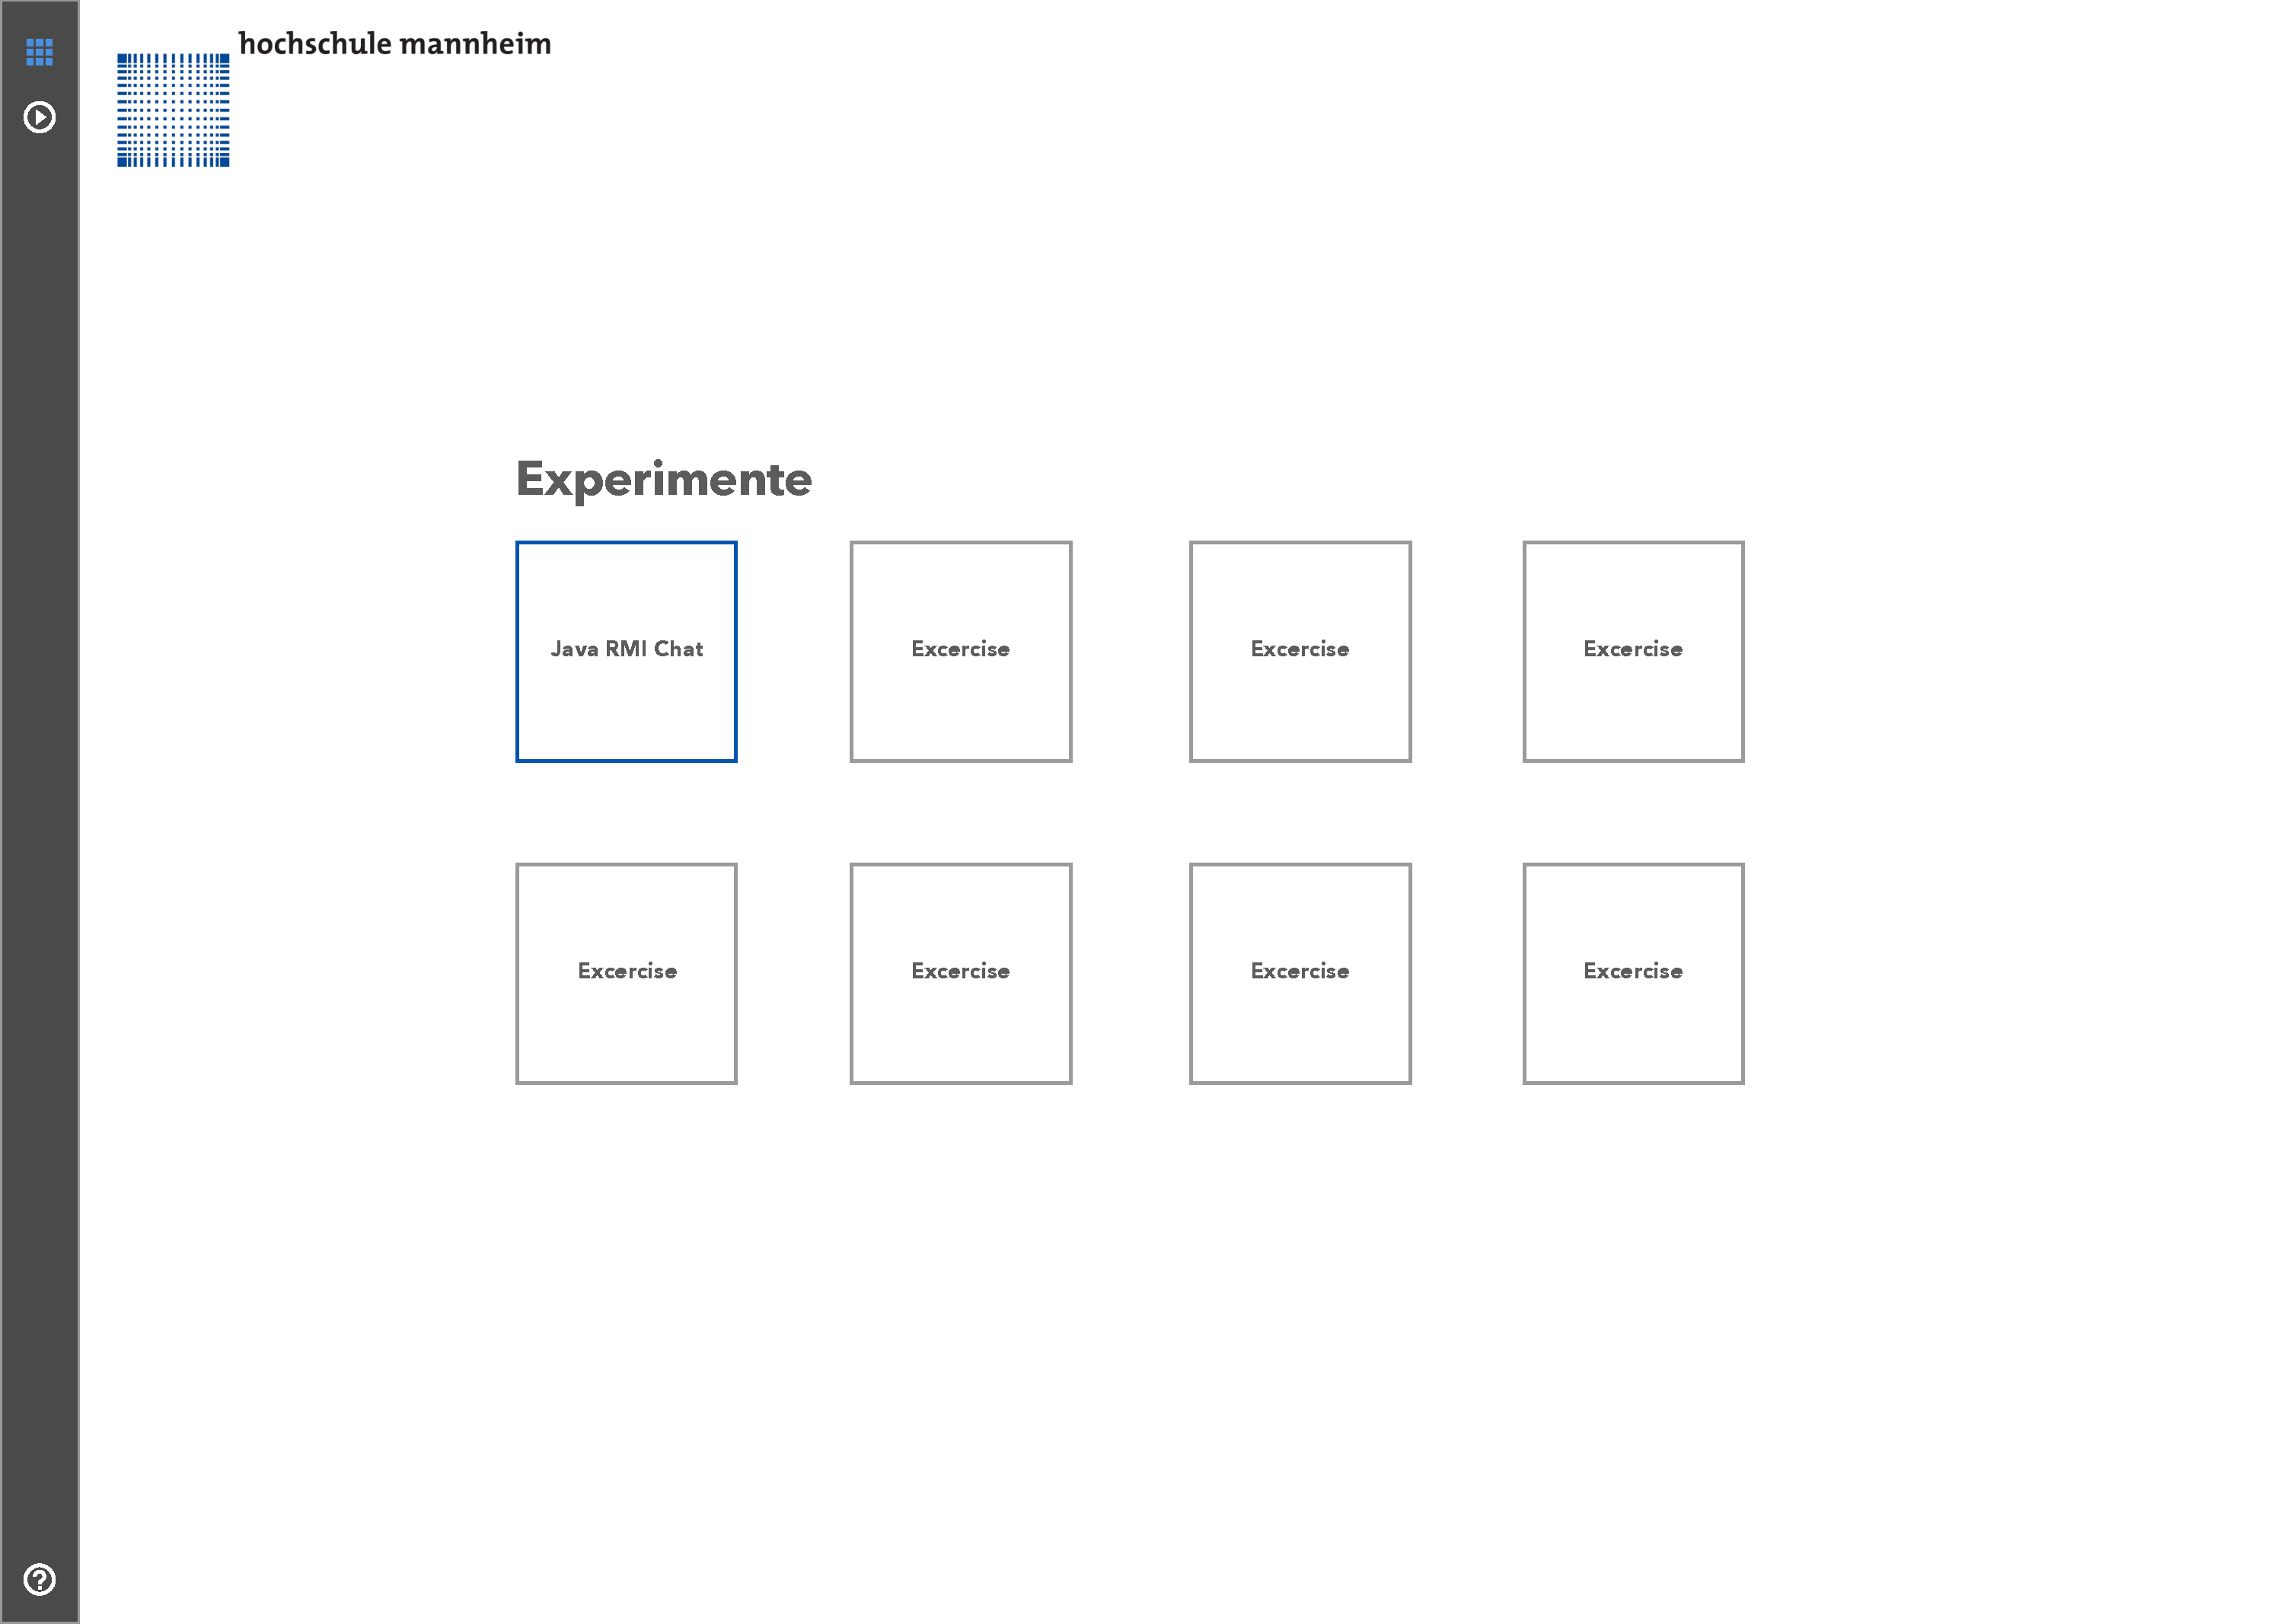
\includegraphics[scale=0.4,page=1]{ui-mockup.pdf}}
    \par
    \caption{UI-Mockup: Übersicht der Experimente}
    \label{fig:ui-mockup-1}
  \end{figure}
  \begin{figure}[h]
    \centering
    \fbox{\includegraphics[scale=0.4,page=2]{ui-mockup.pdf}}
    \par
    \caption{UI-Mockup: Experimentenansicht mit verschiedenen Zuständen pro Instanz}
    \label{fig:ui-mockup-2}
  \end{figure}
\end{landscape}

\section{Architektur}

\subsection{Geschäftsprozesse}
{\bfseries State-Charts}
\begin{landscape}
  \begin{figure}[h]
    \centering
    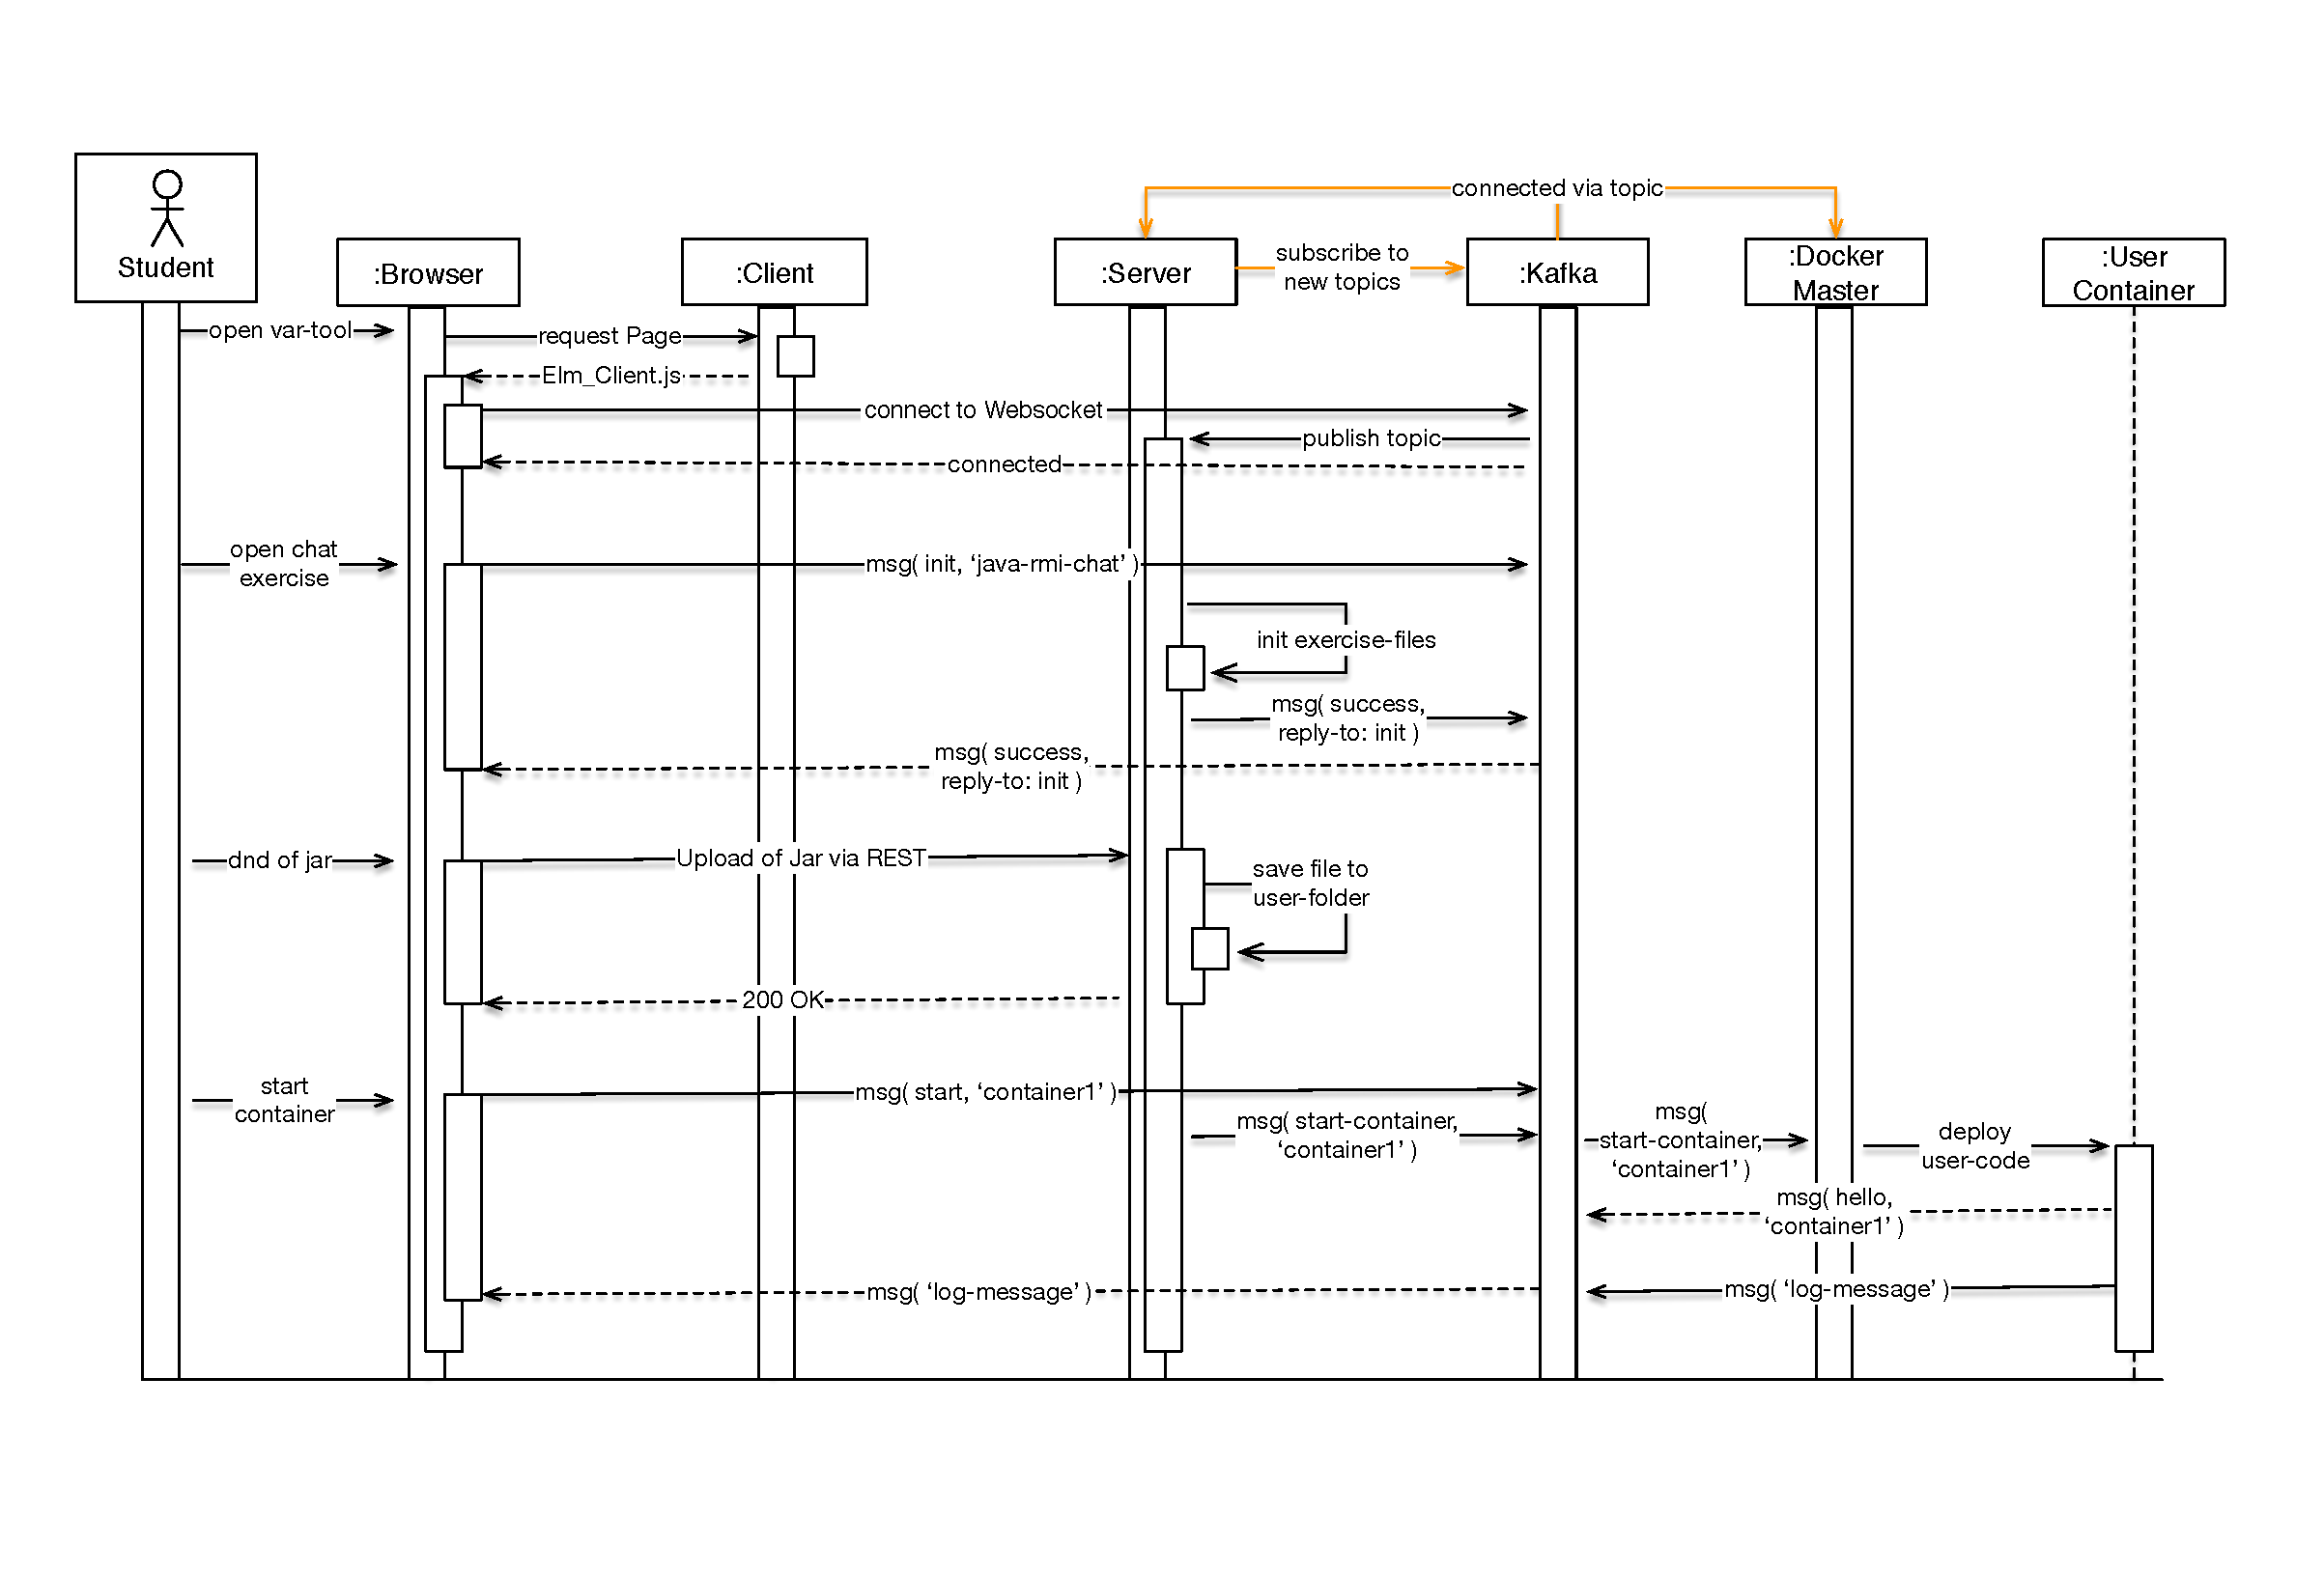
\includegraphics[scale=0.5]{sequence.pdf}
    \par
    \caption{Sequenzdiagramm}
    \label{fig:sequence}
  \end{figure}
\end{landscape}

\subsection{Netzwerkgrenzen}
  \begin{figure}[h]
    \centering
    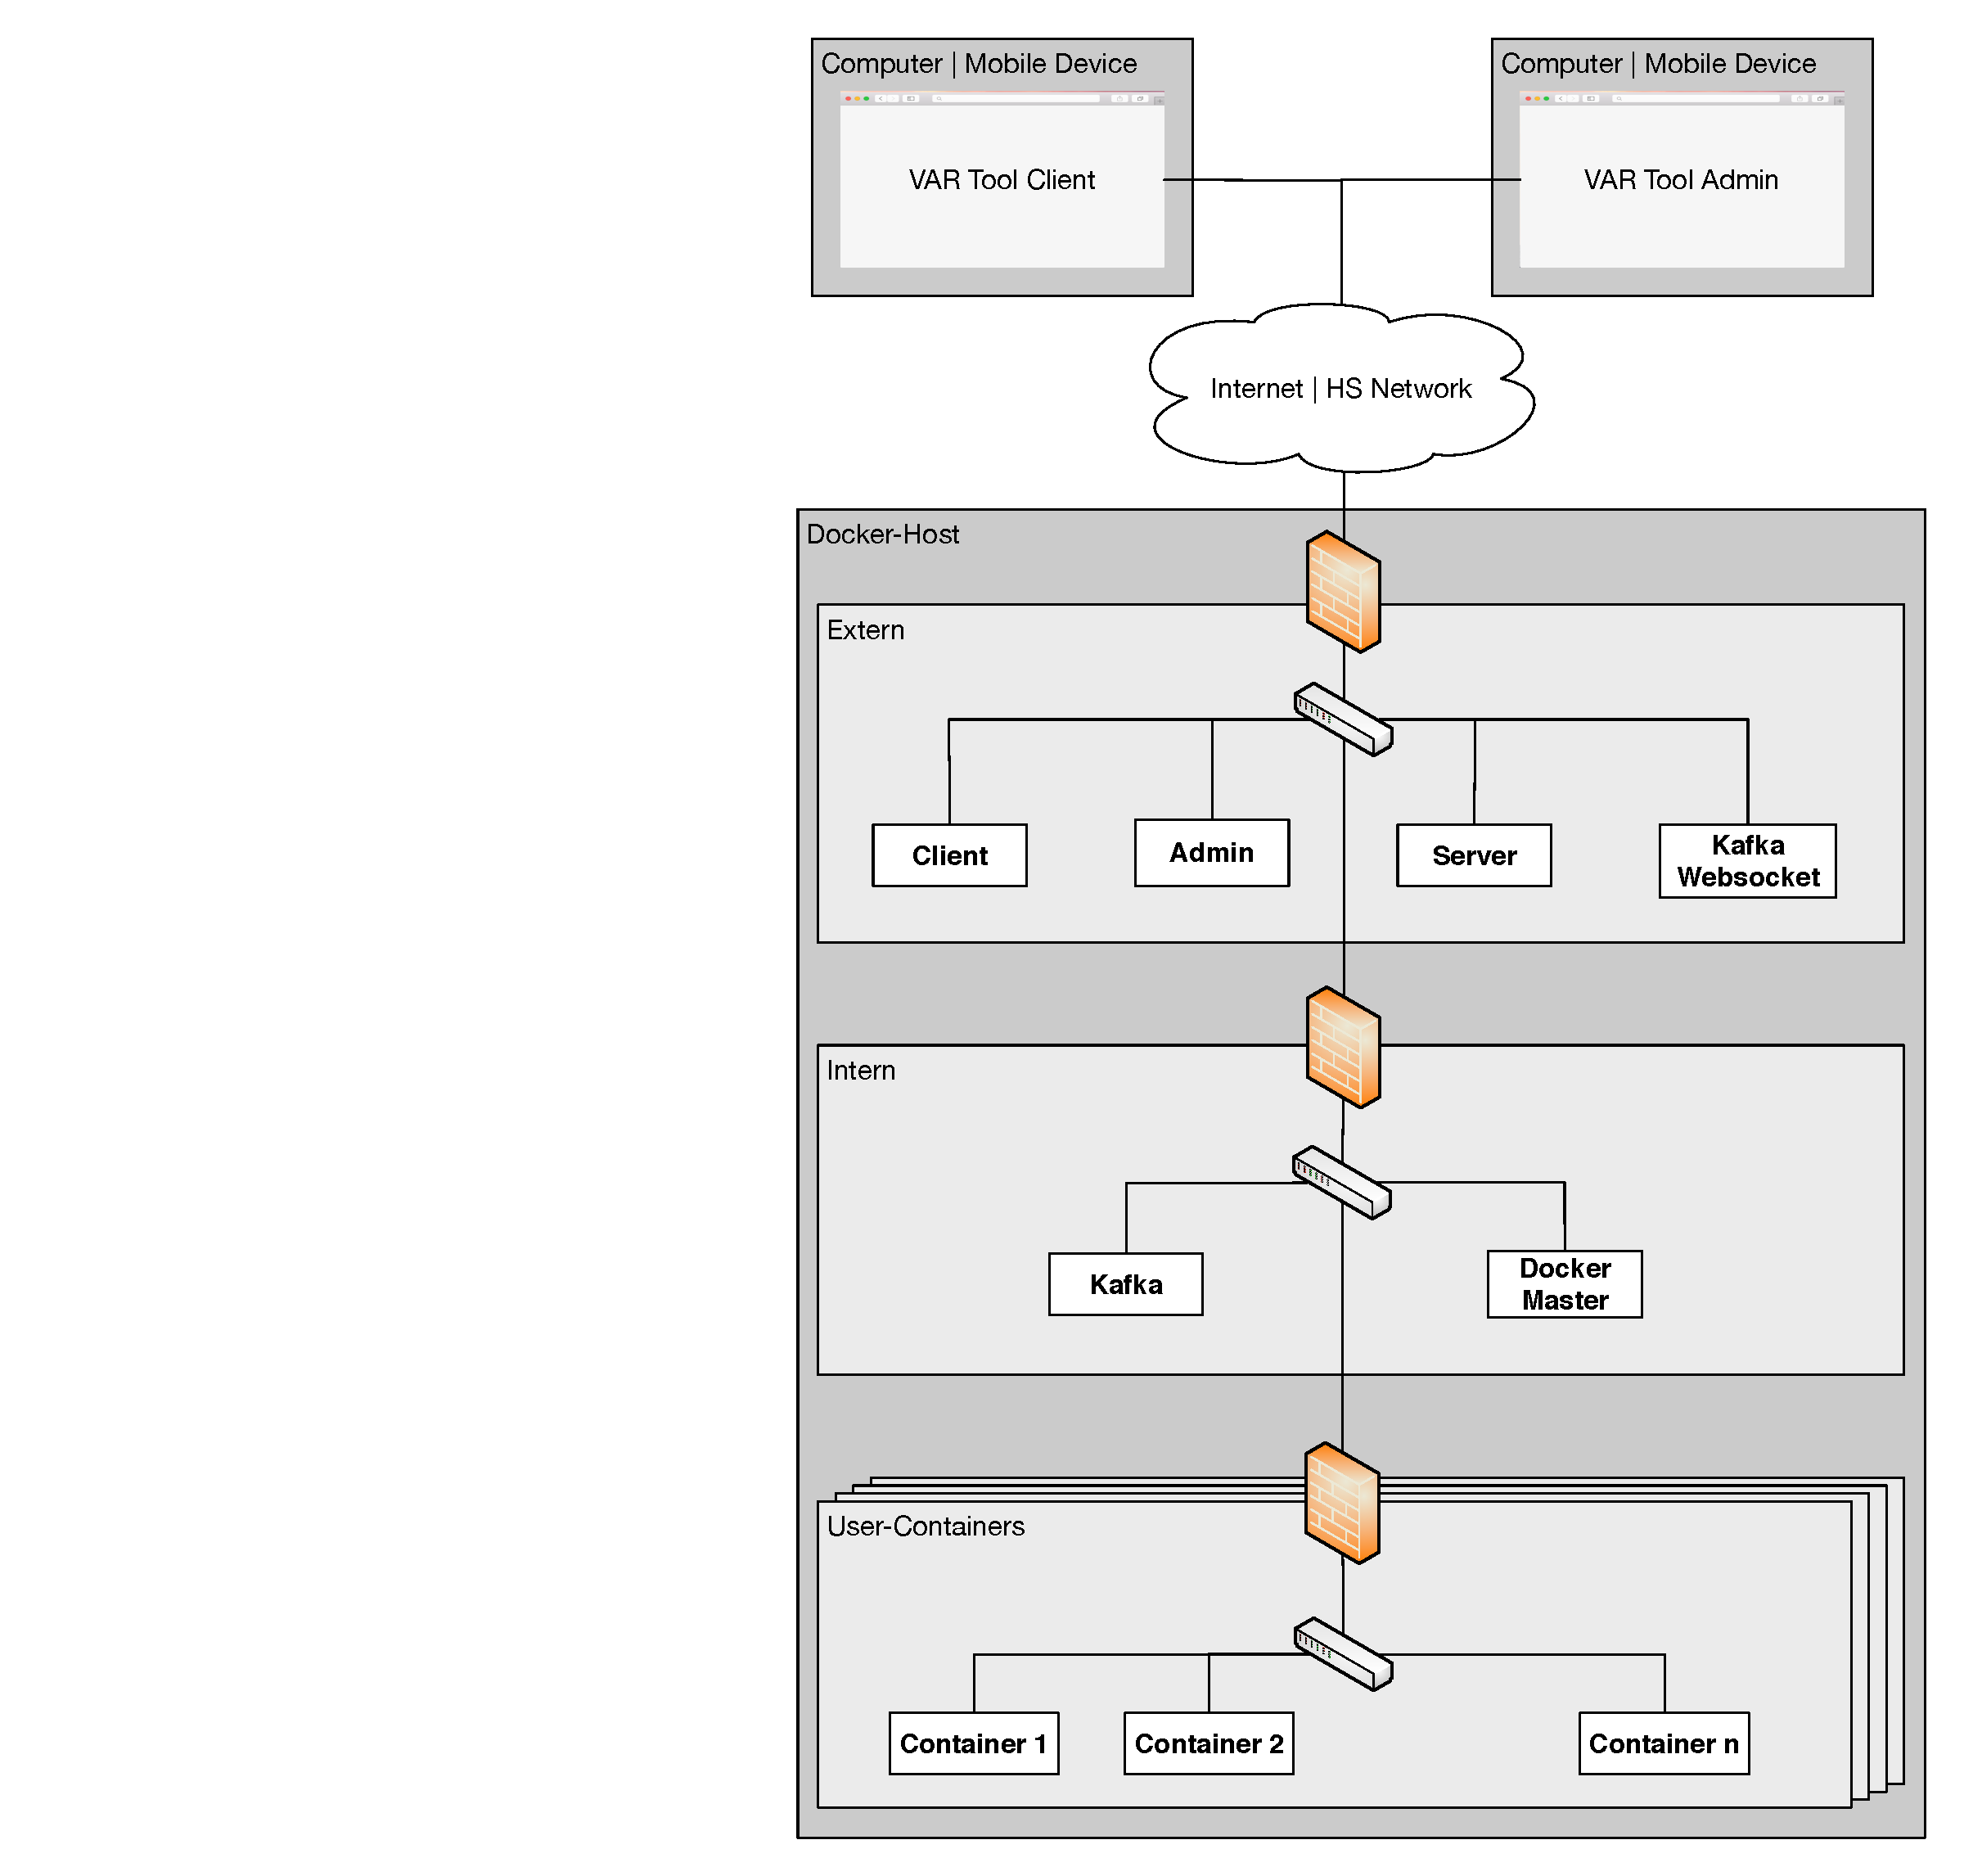
\includegraphics[scale=0.5]{network.pdf}
    % \par
    \caption{Netzwerkdiagramm}
    \label{fig:network}
  \end{figure}
  
Es wird ein Rechner benötigt, welcher aus dem Internet oder hochschulintern erreichbar ist.
  Auf diesem läuft Docker und stellt die Applikation des Projekts bereit.
  Die Zahl an Benutzern des Clients und Admin-Clients ist beliebig, da das Frontend als Web-Applikation realisiert wird.
  \par
  Innerhalb von Docker existieren mehrere gekapselte Netzwerke, welche an einem Bridge-Interface des Docker-Hosts angeschlossen sind.
  Es werden nur solche Ports an den Netzwerken geöffnet, welche in einem Container freigegeben werden.
  Eines dieser Netzwerke stellt die eigentliche Applikation selbst dar und trägt den Namen \textit{vartool\_extern}.
  Ruft ein Studierender das VAR-Tool auf und startet darin eine Instanz eines Experiments, so wird ein neues Netzwerk angelegt.
  Dieses Netzwerk ist unabhängig von anderen Experimenten des gleichen und verschiedenen Studierenden, mit dem Namen \textit{vartool\_\{sessionToken\}\_\{experimentId\}}. 


\subsection{Deployment}
Abbildung~\ref{fig:deployment} zeigt die Verteilung der einzelnen Bestandteile der Applikation.
Die Container Server, User und die Clients werden mithilfe von Docker auf einem Linux-Rechner deployed.
\par
Der Client und Admin-Client bestehen jeweils aus dem Webserver \textit{nginx}, welcher ein statisches HTML-Dokument und ein Java-Script Bundle ausliefert, welches aus einer kompilierten Elm-Applikation resultiert.
Wird die URL eines Clients von einem beliebigen Rechner mit aktuellem Browser aufgerufen, so werden die benötigten Dateien übertragen und die Elm-App gestartet.
Während der Laufzeit des Clients verbindet sich der jeweilige Browser mit dem Server über einen Websocket.
Programmpakete welche hochgeladen werden sollen, werden über REST übertragen.
Es können dort anschließend verschiedene Experimente angezeigt und bei dessen Ausführung seine Ausgaben dargestellt werden.
Im Admin-Client sollen Statistiken dargestellt werden, welche u.A. die aktuelle Anzahl an experimentierten Studierenden umfasst.
\par
Der Server besteht aus einer Java-Umgebung, welche ein Jar mit Clojure-Code ausführt.
Er hat die Aufgabe, einen Websocket-Endpoint anzubieten, welcher die Clients zur Kommunikation nutzen.
Ebenso soll dieser ein Endpoint anbieten, welcher ein Upload von Programmpaketen der Studierenden per POST-Request annimmt.
Jeder Benutzer bekommt einen temporären Ordner zugewiesen, in welchem seine Dateien gespeichert werden sollen.
Dieser User-Ordner werden anschließend für die zugewiesenen User-Container eines jeweiligen Studierenden verfügbar sein.
Mit diesem Seiteneffekt, über das File-System des Docker-Hosts, kann ein User-Container auf die jeweiligen Programmpakete zugreifen und diese ausführen.
\par
Ein solcher Container kann von dem Server gestartet werden, da der Server auf den Docker-Socket des Hosts zugreifen darf.
Sowohl die Eingaben wie auch resultierende Ausgaben sollen zunächst auch über das File-System zwischen Server und einzelnem User-Container geteilt werden.
Der Server reagiert auf die Änderung der Datei und schickt die Ausgaben an den Client.

\begin{landscape}
  \begin{figure}[h]
    \centering
    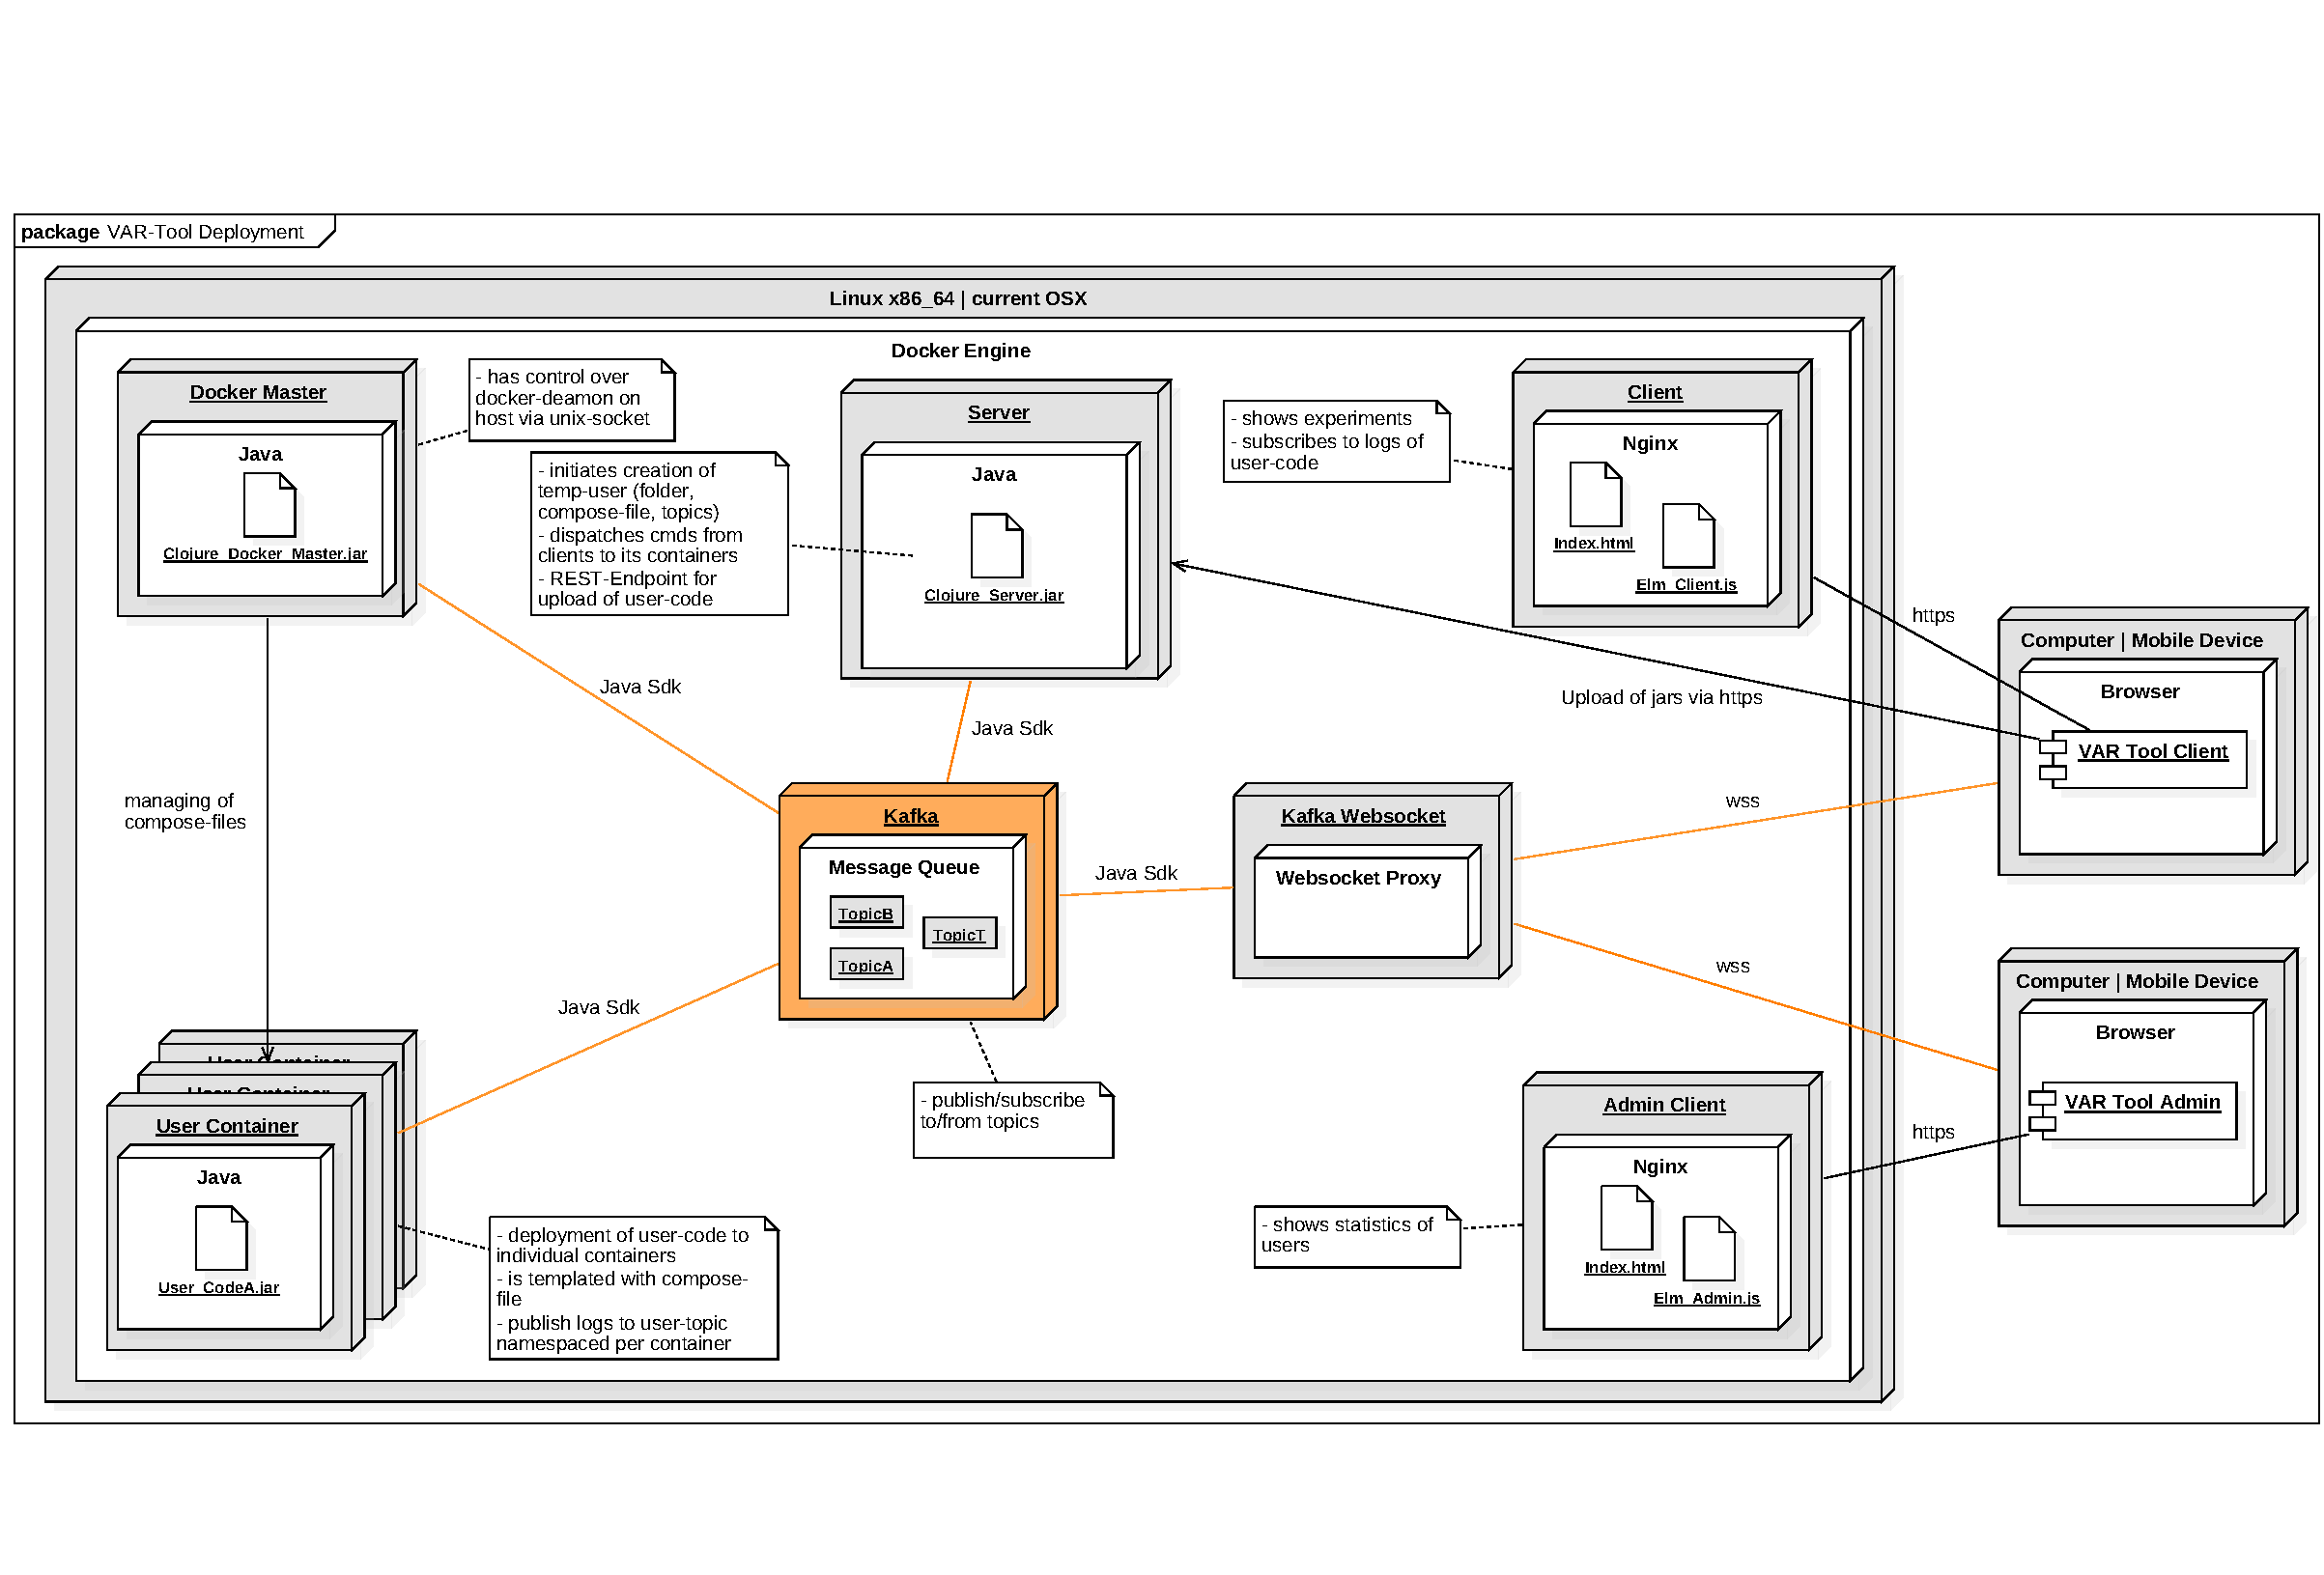
\includegraphics[scale=0.4]{deployment.pdf}
    \caption{Deploymentdiagramm}
    \label{fig:deployment}
  \end{figure}
\end{landscape}

\section{Umsetzung}
Im Folgenden werden Code-Beispiele gezeigt, welche in ihrem vollem Umfang im Repository des Projekts\footnote{\url{https://github.com/jwillem/var-tool}} zu finden sind.
\subsection{Kommunikation über Nachrichten}
Im Vorfeld wurde ein Nachrichten-Protokoll definiert, welches die Kommunikation zwischen Server und Client standardisiert.
Dabei heißen Client-Nachrichten \textit{Commands} und Server-Nachrichten \textit{Messages}.
So können beide Nachrichten-Typen durch ein triviales Merkmal unterschieden werden.
Jeweilig unterscheiden sich diese weiter in Kinder-Typen und deren \textit{Payloads}.
Dabei werden die Daten über eine Websocket-Verbindung in einem JSON-Envelope als String übertragen.
\\\\
\textbf{Commands:}
\begin{itemize}
  \item request-experiments:
    \\\texttt{\{ kind: command, \\subkind: request-experiments \}}
  \item add-input:
    \\\texttt{\{ kind: command, \\subkind: add-input,
    \\ payload: \{ experimentId: rmichat, \\\hspace*{1.8cm}instanceId: 1, \\\hspace*{1.8cm}input: Hello \}\}}
  \item start-instance:
    \\\texttt{\{ kind: command, \\ subkind: start-instance,
    \\ payload: \{ experimentId: rmichat, \\\hspace*{1.8cm}instanceId: 1, \\\hspace*{1.8cm}mainClass: var.rmi.chat.ChatClient, \\\hspace*{1.8cm}arguments: Anton \}\}}
  \item stop-instance:
    \\\texttt{\{ kind: command, \\ subkind: stop-instance,
    \\ payload: \{ experimentId: rmichat, instanceId: 1 \}\}}
\end{itemize}
\textbf{Messages:}
\begin{itemize}
  \item log:
    \\\texttt{\{ kind: message, \\subkind: log,
    \\ payload: \{ experimentId: rmichat, \\\hspace*{1.8cm}instanceId: 1, \\\hspace*{1.8cm}log: Hello\}\}}
  \item reply:
    \\\texttt{\{ kind: message, \\subkind: reply,
      \\ payload: \{ \\\hspace*{0.8cm}to: request-experiments, \\\hspace*{0.8cm}success: true, \\\hspace*{0.8cm}data: \{ \\\hspace*{1.6cm}rmichat: \{ \\\hspace*{2.4cm}id: rmichat, \\\hspace*{2.4cm}name: RMI Chat, \\\hspace*{2.4cm}lecturer: Sandro Leuchter, \\\hspace*{2.4cm}class: VAR, \\\hspace*{2.4cm}numberOfInstances: 4, \\\hspace*{2.4cm}instances: \{ \\\hspace*{3.2cm}1: \{ \\\hspace*{4cm}mainClass: var.rmi.chat.ChatClient, \\\hspace*{4cm}arguments: '' \\\hspace*{3.2cm}\}, .. \\\hspace*{2.4cm}\}\\\hspace*{1.6cm}\}, ..\\\hspace*{0.8cm}\}\\\}}
\end{itemize}
\clearpage

\subsection{Server}
Der Server besteht im Wesentlichen aus einem Webserver basierend auf \textit{http-kit} und \textit{ring} in der Programmiersprache Clojure.
Um die Entwicklung zu vereinfachen, wurde als erster Schritt ein Development-Container in Docker erstellt, welcher sich bei einer Änderung einer Quellendatei selbst aktualisiert, ohne die Java-VM neu zu starten.
\\\\
Es gibt dort drei Endpoints:
\begin{itemize}
  \item GET: \texttt{server:8080/hello}
    \\ Ankündigen des Clients am Server, Empfangen eines Responses mit \texttt{Set-Cockie}-Header
  \item \texttt{ws://server:8080/ws}
    \\ Anmeldung von Client an Websocket, Senden und Empfangen von Nachrichten
  \item POST: \texttt{server:8080/experiment/\{experimentId\}/instance/\{instanceId\}}
    \\ Hochladen der Programmpakete eines Studierenden; Werden in temporären User-Ordner in \texttt{data/submissions/\{session-token\}/\break\{experimentId\}/\{instanceId\}/\{fileName\}} gespeichert
\end{itemize}
% \clearpage
Um auf eintreffende Nachrichten zu reagieren (\texttt{on-receive}), wurde eine \texttt{match}-Funktion innerhalb des Websocket-Handler genutzt (Listing 3.1).
Zu- nächst werden die Nachrichten von ihrer Json-Repräsentation in ein für Clojure passendes Keyword decodiert.
Weiterhin wird auf eine passende verarbeitende Funktion verwiesen, oder einen Fehler mithilfe von \texttt{handle-\break command-error} an den Websocket-Channel zurückgegeben.
\par Bei einem Eintreffen eines \texttt{start-instance}-Commands wird ein Docker-Compose-Template eines Experiments mit den übergebenen Daten (Main-Class \& Argumentenliste) befüllt.
Dies geschieht mit dem Unix-Tool \texttt{envsubst} aus der \texttt{gettext}-Suite, welches Umgebungsvariablen in dem Docker-Compose-Template ersetzt.
Dabei wird die Datei als \texttt{docker-compose.yml} in dem Datenverzeichnis \texttt{data/submissions/\{session-token\}/\{experimentId\}/} des Projekts gespeichert und ausgeführt (\texttt{docker-compose run user\_\break\{instanceId\}}).
Es wird zum Ausführen der jeweiligen Instanz das vorher hochgeladene Programmpaket in einem Unterordner mit dem Namen der Instanz-Id verwendet. 
\\\\
Um ein Experiment zu definieren wurde folgendes Konzept erarbeitet:
\begin{itemize}
  \item \texttt{data/experiments/\{experimentId\}/} \\dient als ein Entry-Point um portable „self-contained“ Experimente zu enthalten.
  \item \texttt{data/experiments/\{experimentId\}/experiment.yml} \\enthält einige beschreibende Eigenschaften eines Experiments.
    Diese können später im Client genutzt werden.
  \item \texttt{data/experiments/\{experimentId\}/docker-compose.yml.template} \\beschreibt ein Experiment über enthaltene Services mit seinen spezifizierten Eigenschaften der \texttt{user\_\{instanceId\}}-Containern.
    Es können dort auch andere für die Lösung der Aufgabe nötigen Dienste aufgeführt werden.
  \item \texttt{data/experiments/\{experimentId\}/user/Dockerfile} \\kann optional in Docker-Compose-Templates genutzt werden, um besondere Konfigurationen an einem Containersystem vornehmen zu können.
    Das Beispiel Template nutzt zurzeit das Docker-Image \texttt{openjdk:8}, das beschriebene Dockerfile erbt ebenfalls von diesem.
  \end{itemize}
  Das Parsen eines \texttt{experiment.yml} erfolgt im Moment noch nicht, ist aber bei geringem Aufwand realisierbar.
  Die im Client angezeigten Experimente sind in der Datei \texttt{server/src/var\_tool/server/fixtures.clj} definiert.
  Natürlich sei es dahingestellt, ob das Austauschformat der Experimente als Yaml oder als Clojure-Keyword sinnvoller erscheint.

\clearpage
\begin{verbatim}
(defn websocket-handler
  ""
  [request]
  (with-channel request channel
    (on-close
      channel
      (fn [status] (println "channel closed: " status)))
    (on-receive
      channel
      (fn [data]
        (let [session-token (get-in request [:cookies "ring-session" :value])
              ;; TODO error if session-token empty
              ;; TODO return error on java.lang.Exception: JSON error
              command-keyword (json/read-str data :key-fn keyword)
              _ (println "new command: " command-keyword)
              {:keys [kind subkind payload]} command-keyword]
          (match [kind subkind]
                 ["command" "request-experiments"]
                   (handle-request-experiments channel)
                 ["command" "add-input"]
                   (handle-add-input channel payload session-token)
                 ["command" "start-instance"]
                   (handle-start-instance channel payload session-token)
                 ["command" "stop-instance"]
                   (handle-stop-instance channel payload session-token)
                 :else (handle-command-error channel)))))))
\end{verbatim}
\begin{center}
  Listing 3.1: Websocket-Handler im Server (\texttt{handler.clj})
\end{center}
\clearpage

\subsection{Client}
Der Client wurde in der Programmiersprache Elm erstellt und nutzt \textit{elm-mdl} um die Darstellung aus Elementen im Stile des Material-Design Frameworks von Google aufzubauen.
Auch für den Client wurde zunächst ein Development-Container definiert, welcher automatisch neue Quelldateien kompiliert und den Browser dazu auffordert, sich zu aktualisieren.
\par
Die Entwicklung seiner Funktionen wurde stark durch das Typensystem und den Compiler von Elm geprägt, welche sich als sehr hilfreich herausgestellt haben.
Dazu wurden die Typen in einer Datei \texttt{Types.elm} definiert welche in anderen Elm-Modulen importiert wird.
Bei der Größe des Projektes ist es noch in Ordnung alle Typendefinitionen in einer Datei zu haben, jedoch sollte man diese in Zukunft bedachtsam in Unter-Module aufteilen.
\par
Weiterhin wurden die Json-Encoder definiert, welche ausgehende Nachrichten in eine Json-Repräsentation bringt.
Ebenso war es wichtig eingehende Nachrichten mittels mehrerer Json-Decoder in Elm-Typen zu konvertieren.
Man erlangt so eine strikte Typisierung bei sowohl eingehenden- wie auch  ausgehenden Daten.
Innerhalb dieser, konnte ebenso eine \texttt{match}-Funktion zum Einsatz gebracht werden (Listing 3.2).
Dabei können in einem \texttt{case}-Statement beliebige Elm-Typen auf einen Match überprüft werden.
Im Payload-Decoder wird ein Record vom Typ Message-Base mit dem \texttt{kind} von 'message' und den \texttt{subkind}s von 'log' oder 'reply' erwartet.
Im Code-Beispiel ist ebenso der Log-Payload-Decoder aufgeführt, welcher schließlich eine Log-Message zurückgibt.
\par Der vorbereitete Decoder kommt anschließend innerhalb der \texttt{update}-Funktion von \texttt{Update.elm} zum Einsatz (Listing 3.3).
Es wird zunächst überprüft, ob die Dekodierung erfolgreich war und anschließend den beiden Message-Typen zugeordnet, welche jeweilig anders mit den übergebenen Daten umgehen.
\par Die Umsetzung der Mockups aus Abbildung~\ref{fig:ui-mockup-1} und~\ref{fig:ui-mockup-2} sind in den Abbildungen~\ref{fig:dev-view-1} und~\ref{fig:dev-view-2} zu erkennen.
Dabei wurde versucht möglichst alle initialen Ideen zu erhalten und einige Verbesserungen integriert.
So war in den Mockups vorherig kein Eingabefeld vorhanden, um Eingaben an die laufenden Programme zu senden.
Weiterhin wurden die Zustände der Instanzansichten vereinfacht. Es sind nun folgende Zustände möglich:
\begin{itemize}
  \item Empty
    \\ Zeigt den File-Uploader
    (Abb.~\ref{fig:dev-view-2} links oben)
  \item Uploading
    \\ Zeigt eine Warteinformation beim Hochladen der Programmpakete
    (Abb.~\ref{fig:dev-view-2} rechts oben)
  \item Settings
    \\ Zeigt die Start-Parameter der Instanz
    (Abb.~\ref{fig:dev-view-2} links unten)
  \item Running
    \\ Zeigt die Logs einer laufenden Instanz
    (Abb.~\ref{fig:dev-view-2} rechts unten)
\end{itemize}
Die Darstellung der Instanzen aus Abbildung~\ref{fig:dev-view-2} ist dynamisch, d.h. die Höhe der angezeigten Instanzen passt sich je nach Instanzanzahl eines Experiments an.
Somit wird die verfügbare Fläche des Browserfensters optimal genutzt.
\par
Die Dateiauswahl innerhalb einer Instanz (Instanz hat den Zustand \texttt{Empty}) könnte in Zukunft bei geringem Aufwand einen Drag-and-Drop-Container erhalten, welcher das Hochladen vereinfachen würde. 
\par Die angezeigten Experimente in Abbildung~\ref{fig:dev-view-1} werden bei einem Neustart der Applikation über die bestehende Websocket-Verbindung abgefragt (request-experiments).
Die dabei erhaltenen Daten werden im Browser-Cache gespeichert und können nach einem Auswählen eines Experiments wiederverwendet werden.
\par
Der geplante Admin-Client konnte aus zeitlichen Gründen nicht mehr entwickelt werden.
Die Übermittlung der Daten kann analog mit der oben entwickelten Methode über ein Command im Client bzw. einem Reply im Server geschehen.
Die im Admin-Interface anzuzeigenden Daten müssten ebenso noch im Server gesammelt werden.
\clearpage
\begin{verbatim}
messageDecoder : Decoder Message
messageDecoder =
    map2 MessageBase
        (field "kind" string)
        (field "subkind" string)
        |> andThen payloadDecoder

payloadDecoder : MessageBase -> Decoder Message
payloadDecoder { kind, subkind } =
    case kind of
        "message" ->
            case subkind of
                "log" ->
                    field "payload" logPayloadDecoder

                "reply" ->
                    field "payload" replyPayloadDecoder

                _ ->
                    fail "Subkind is unknown!"

        _ ->
            fail "Kind is unknown!"


logPayloadDecoder : Decoder Message
logPayloadDecoder =
    map3 LogPayload
        (field "experimentId" string)
        (field "instanceId" string)
        (field "log" string)
        |> andThen logMessageDecoder


logMessageDecoder : LogPayload -> Decoder Message
logMessageDecoder payload =
    succeed (LogMessage payload)
\end{verbatim}
\begin{center}
  Listing 3.2: Json-Decoder der Log-Messages im Client (\texttt{Decoders.elm})
\end{center}
\clearpage
\begin{verbatim}
handleNewMessage : Model -> String -> ( Model, Cmd Msg )
handleNewMessage model message =
    let
        decodedMessage =
            Decoders.decodeMessage message
    in
        case decodedMessage of
            Ok message ->
                case message of
                    LogMessage payload ->
                        handleLogMessage model payload

                    DataMessage payload ->
                        handleDataMessage model payload

            Err error ->
                let
                    _ =
                        Debug.log "Decoder" error
                in
                    ( model, Cmd.none )
\end{verbatim}
\begin{center}
  Listing 3.3: Verarbeiten von neuen Nachrichten im Client (\texttt{Update.elm})
\end{center}

\begin{landscape}
  \begin{figure}[h]
    \centering
    \fbox{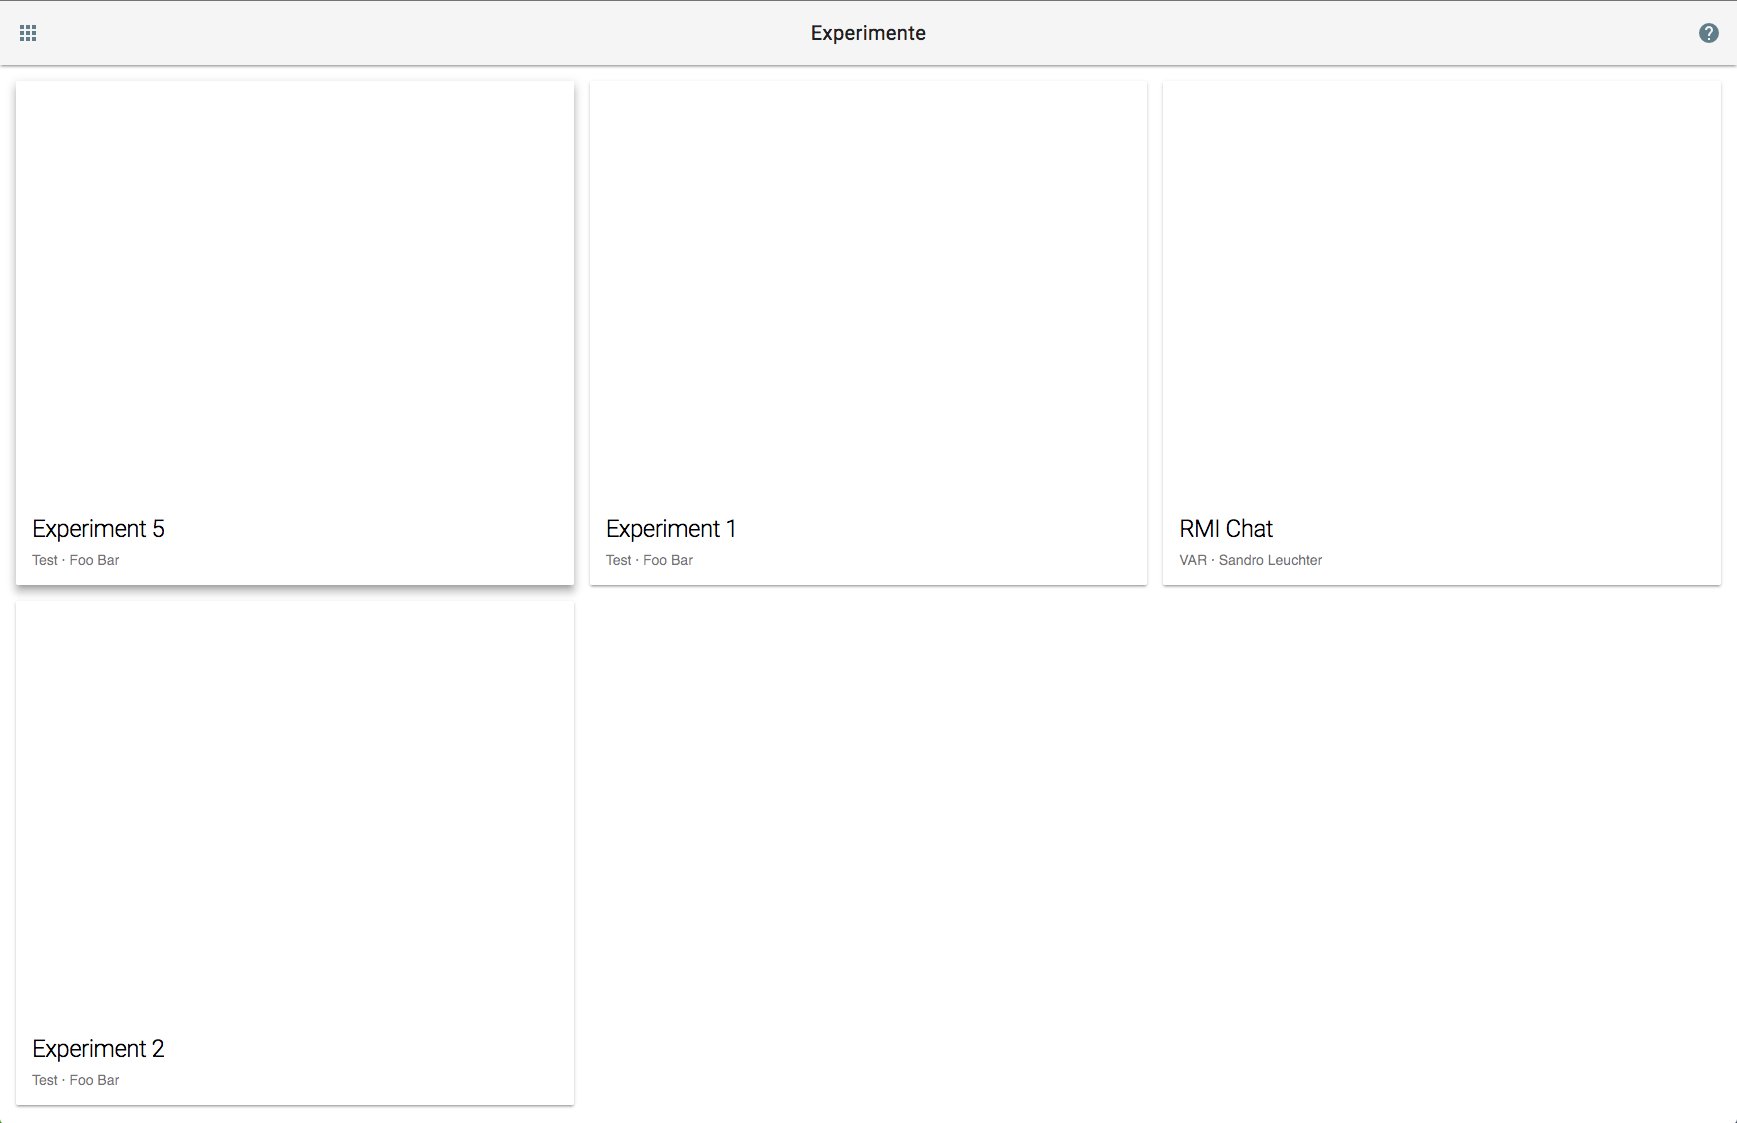
\includegraphics[scale=0.35]{current_dev_view_overview.png}}
    \par
    \caption{Umsetzung des Clients: Übersichtsseite}
    \label{fig:dev-view-1}
  \end{figure}
  \begin{figure}[h]
    \centering
    \fbox{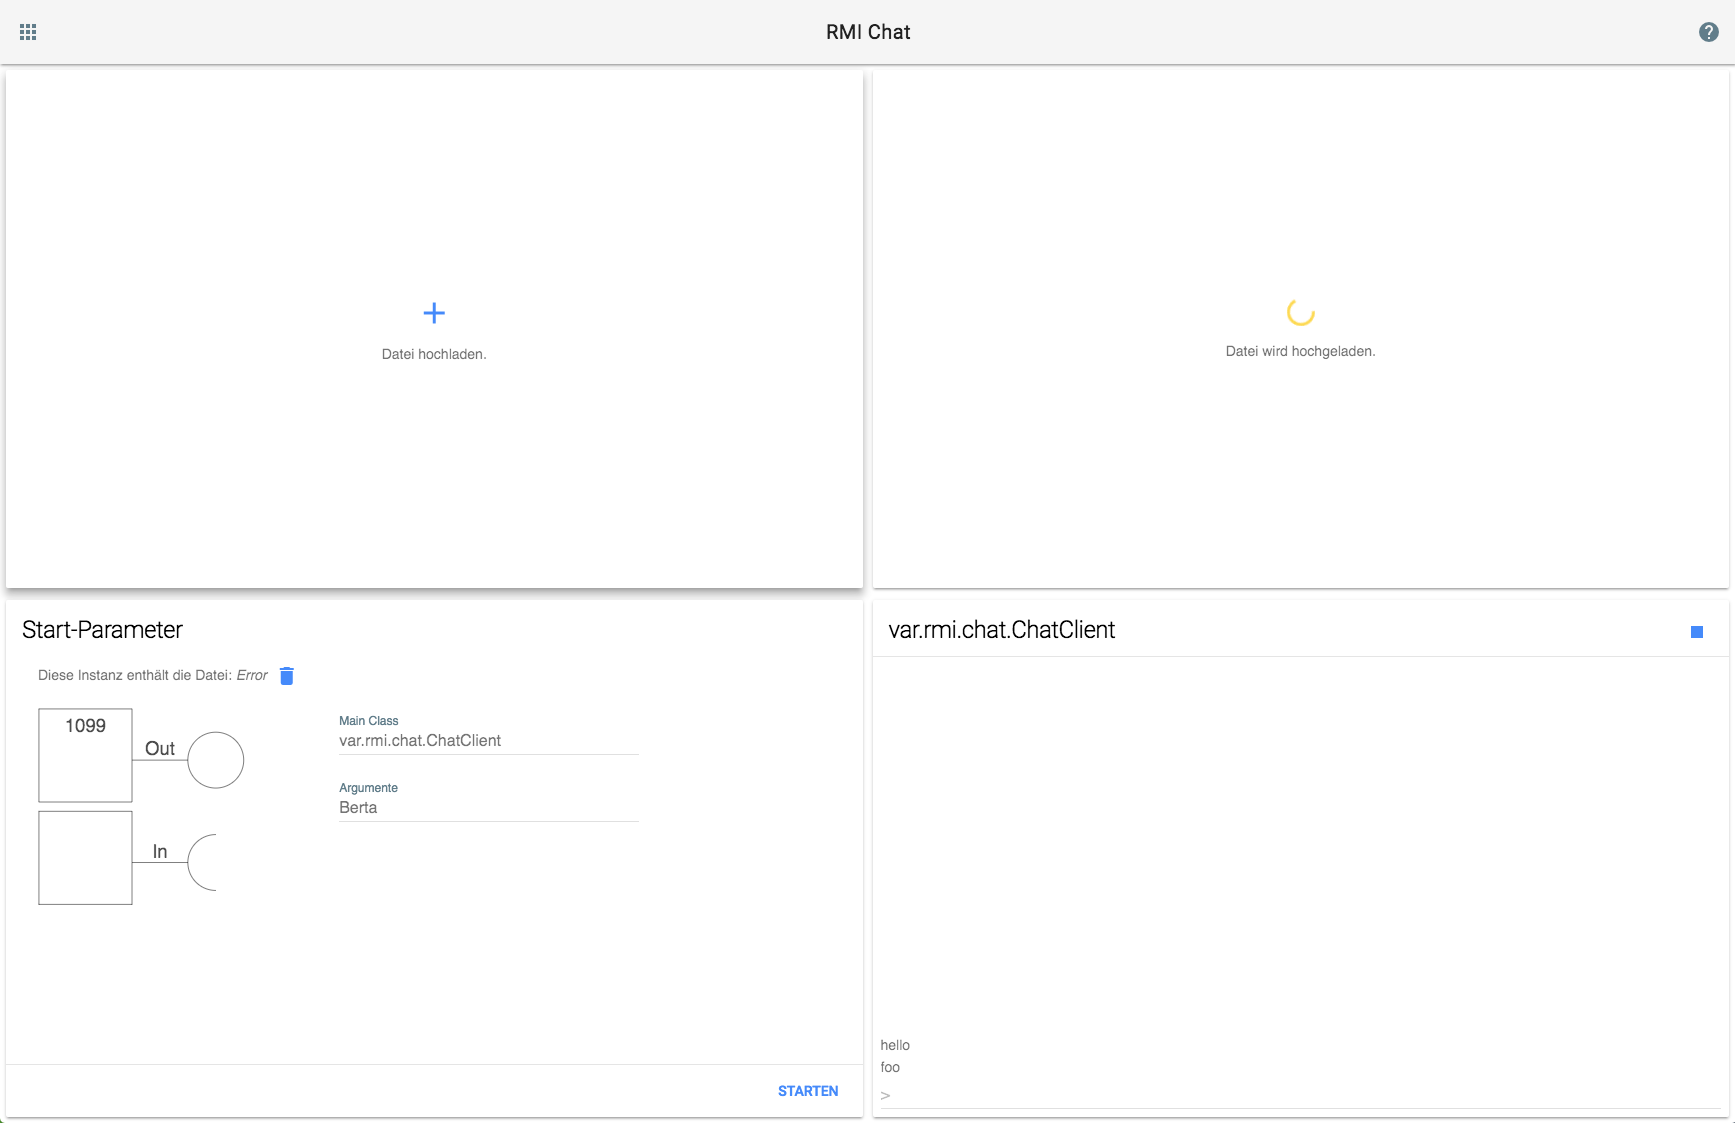
\includegraphics[scale=0.35]{current_dev_view_experiment.png}}
    \par
    \caption{Umsetzung des Clients: Experimentenansicht}
    \label{fig:dev-view-2}
  \end{figure}
\end{landscape}
\section{Erwartungen an die Performance}
Der Client ist über einen Websocket mit dem Server verbunden.
D.h. bei einer stabilen Internetverbindung sollten auftretende Logs innerhalb von wenigen Sekunden im Client sichtbar sein.
Dies ist möglich, da der Client nicht in einem bestimmten Interval nach neuen Logs frägt, sondern aktiv davon benachrichtigt wird.
\\
Auf Seiten der User-Container werden die Logs in eine Datei geschrieben und damit gepuffert.
Der Server wartet auf Änderungen an dieser Datei und gibt die Inhalte an den Client weiter.
Die Kopplung der User- und Server-Container über die Dateiebene sollte keine Performanceeinbußen bedeuten.
\section{Installation}
Als erstes wird das Projekt mithilfe von \texttt{git clone \url{https://github.com/jwillem/var-tool.git}} heruntergeladen.
Um die Applikation zu starten, werden zunächst die Installationen von Docker\footnote{\url{https://www.docker.com/community-edition}} und Docker-Compose\footnote{\url{https://docs.docker.com/compose/install/}} benötigt.
Nach einem Ausführen von \texttt{docker-compose build} im Projektverzeichnis kann die App mit \texttt{docker-compose up} gestartet werden.
\\
Sollte eine weitere Entwicklung erfolgen, so können die vorbereiteten Development-Container genutzt werden.
Dazu führt man \texttt{docker-compose -f docker-compose\break .dev.yml up} aus.
